\chapter{Our solution} \label{our:solution}
% TODO insert \nopagebreak after \midrule s

In our solution we design an AutoML system for workflow optimization based on
developmental genetic programming. Compared to existing systems it supports 
arbitrary-sized pipelines as well as complex ensemble structures. An overview
of the process is shown in algorithm \ref{alg:genens}. In section
\ref{genens:devGP} we describe how we apply the developmental GP to this
problem (line \ref{line:devGP}). Evaluation of pipelines (line \ref{line:compile})
and implementation details as well as relation to scikit-learn
(\cite{scikit-learn}) are presented in section \ref{genens:eval}.

\begin{algorithm}
\DontPrintSemicolon 
\caption{Pipeline optimization --- main\label{alg:genens}}
  \KwData{dataset $d$, configuration $c$}
  \KwResult{optimized pipelines}
  \SetKwFunction{Compile}{Compile}
  \;
  $individuals \longleftarrow$ run developmental GP on $d$ with $c$ \label{line:devGP} \;
  $pipelines \longleftarrow$ \Compile{$individuals$} \label{line:compile}
  \;\;
  \KwRet{pipelines}
  
\end{algorithm}

% POHLED ZVRCHU shrnout vse, detaily dole

% indiv. preloz do sklearn pipeliny, evaluuj ji na datech


\section{Evolutionary optimization of pipelines} \label{genens:devGP}
In this section, we describe the necessary components of the evolutionary algorithm.
The process corresponds to the schema of a general evolutionary algorithm
\ref{alg:EA}. A more detailed schema is presented in algorithm \ref{alg:devgp}.
Individuals of this particular EA are pipelines encoded as trees via
developmental GP; the encoding is summarized in section \ref{sec:encoding}.
The initialization procedure (line \ref{alg:genens:init}) is explained in
section \ref{sec:init}. All reproduction operators
(line \ref{alg:genens:repro}) are presented in section \ref{sec:repro}.
Finally, the selection and fitness are specified in section \ref{sec:fitsel}
(lines \ref{alg:genens:genvalid} and \ref{alg:genens:nsga}).


\begin{algorithm}
{\small

\DontPrintSemicolon 
\caption{Pipeline optimization --- developmental GP \label{alg:devgp}}
  \KwData{population size $k$, maximum number of generations $max\_gen$,
  crossover probability $p_{cx}$,
  mutation probabilities $p_{mut}$, $p_{mut\_node}$, $p_{mut\_args}$ }
  \KwResult{evolved tree individuals}
  \SetNoFillComment
  \SetKwFunction{Cx}{crossover}
  \SetKwFunction{Mut}{mutation}
  \SetKwFunction{Mutnode}{node\_mutation}
  \SetKwFunction{Mutarg}{arg\_mutation}
  \SetKwFunction{Eval}{evaluate}
  \SetKwFunction{Compile}{compile}
  \SetKwFunction{GenValid}{generate\_valid}
  \;
 
  \Fn{\Eval}{ \label{alg:genens:eval}
        $pipe \longleftarrow$ \Compile($ind$) \;
        $score, time \longleftarrow$ cross-validate $pipe$ on a sample\;
        $ind.fitness \longleftarrow (score, \log\mleft(time\mright))$
  }
  \;
  \Fn{\GenValid}{
  		\While{$score$ is not valid}{
           $ind \longleftarrow$ initialize a new individual\;
           $score \longleftarrow$ \Eval{ind}
        }
  }  
  \;  
  \tcc{run developmental GP}  
  $P(0) \longleftarrow$ initialize population of GP trees \label{alg:genens:init}
  \;\;
  \While{$n < max\_gen$}{
      \;
      \tcc{compute fitness of population}
      \For{$ind$ in $P(n)$} {  \label{alg:genens:genvalid}
         \Eval{$ind$}\;
         \If{fitness is not valid}{
             \GenValid{$ind$}
         }
      }
      \;
      \tcc{reproduction} \label{alg:genens:repro}
      \For{$i$ in \Range{$k/2$}} {
         $i_1, i_2 \longleftarrow$ tournament selection from $P(n)$

         \If{$p_{cx}$} {
            \Cx{$i_1$, $i_2$} \tcc*[r]{subtree crossover}
         }
         \;
         \If{$p_{mut}$ for $k=1,2$} {
            \Mut{$i_k$} \tcc*[r]{subtree mutation}
         }
         \If{$p_{mut\_node}$ for $k=1,2$} {
            \Mutnode{$i_k$} \tcc*[r]{node mutation}
         }
         \If{$p_{mut\_args}$ for $k=1,2$} {
            \Mutarg{$i_k$} \tcc*[r]{hyperparameter mutation}
         }
         
         \;
         \If{\Eval{$i_k$} for $k=1,2$}{
             add $i_k$ to offspring population $P_o(n)$
         }
         \Else{
             \GenValid{$i_k$} and add to $P_o(n)$
         }
      }
      \;
      $P(n+1) \longleftarrow$ NSGA-II selection from $P_o(n)$ \label{alg:genens:nsga} \;
  }
  \;
  \KwRet{Pareto front of $P(c)$} 

}
\end{algorithm}


\subsection{Individual encoding} \label{sec:encoding}
\begin{figure}[ht]\centering
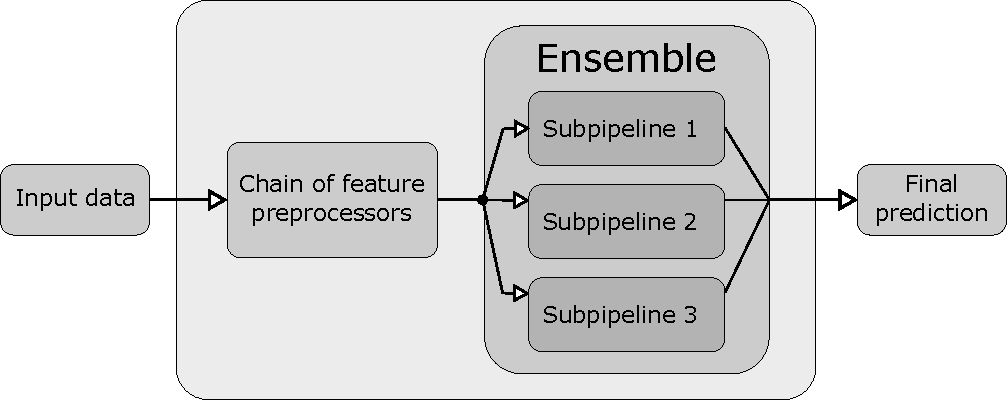
\includegraphics[width=0.7\textwidth]{../img/pipeline-pdfa.pdf}
\caption{Schema of an example pipeline}
\label{pic02:pipeline}
\end{figure}

The individual encoding is one of the most important parts of this system. With
ensembles and complex feature preprocessing methods like stacking or feature
union, most of the pipelines become in fact directed acyclic graphs (Figure~\ref{pic02:pipeline}). Therefore, we cannot directly use the simple tree-based
encoding. Instead we use the developmental GP with cellular encoding described
in section~\ref{devGP}.

In our case, the embryo is an empty pipeline. To create a complex pipeline, we
modify it by inserting steps into it.

\begin{figure}[ht]\centering
    \subfloat[Tree encoding]{{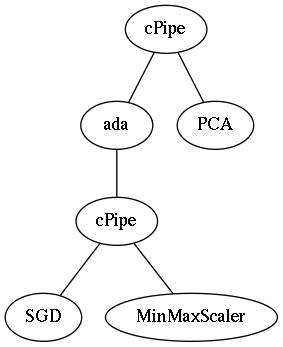
\includegraphics[width=0.25\textwidth]{../img/ada.png} }}%
    \qquad
    \subfloat[Encoded pipeline]{{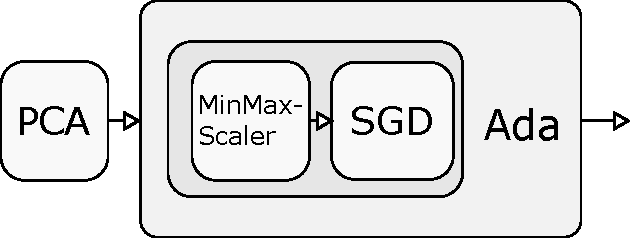
\includegraphics[width=0.5\textwidth]{../img/ada-pdfa.pdf} }}%
    \caption{An example pipeline encoded to a tree individual}%
    \label{pic:pipeencoding}%
\end{figure}

The process can be demonstrated on Figure
\ref{pic:pipeencoding}. The root of the tree represents the embryo which will
be modified by subsequent operations. In this case, the left subtree modifies
the ensemble structure whereas the right subtree modifies the feature
preprocessor chain. The pipeline contains only one preprocessor, hence the
right subtree is terminated by the corresponding node. The left son can be
either an ensemble or a simple method. Here it is the AdaBoost ensemble which
has one base classifier. The subestimator is again a pipeline, which is composed
of a MinMaxScaler and Stochastic gradient descent classifier. The specific
hyperparameter of every pipeline step are stored aside the nodes and are not
depicted in the figures.

\label{sec:decoding}
Table \ref{tab03:nodes} lists all nodes used in the current implementation of
our system. Input type is defined as a cartesian product of types, output type
is a single type; terminals have only the output type defined. Output types of
child nodes must match the input type of parent node. The list is extensible,
it is possible to add a definion of similar nodes, e.g. a different ensemble
flavour like stacking. The nodes that are specific for a given estimator
correspond to the list of methods in section \ref{tab03:methods}. To decode
the pipeline, the tree is traversed from root to leaves while applying the
operations associated with the nodes.

\begin{table}[b!]

\centering
\caption{Nodes representing modifying operations}\label{tab03:nodes}
\begin{tabular}{l c c p{0.38\textwidth}}
\toprule
\mc{\textbf{Node}\textsuperscript{1}} & \mc{\textbf{In type}\textsuperscript{2}} &
\mc{\textbf{Out type}\textsuperscript{3}} & \mc{\textbf{Operation}} \\
\midrule
cPipe       & $ens \times data$      & $out$  & Create pipeline with a preprocessor chain and a predictor \\
cPred       & $ens$                  & $out$  & Create pipeline only with a predictor \\
cData       & $featsel \times scale$ & $data$ & Create preprocessor chain with feature selector and scaler \\
cFeatSelect & $featsel$              & $data$ & Create preprocessor chain only with a feature selector \\
cScale      & $scale$                & $data$ & Create preprocessor chain only with a scaler \\
dUnion      & $data^n$               & $data$ & Create feature union in the preprocessor chain \\
\textit{ensemble} & $out^n$ & $ens$ & Insert ensemble \\
\textit{classifier} & $\emptyset$ & $out$ & Insert classifier \\
\textit{selector} & $\emptyset$ & $featsel$ & Insert feature selector \\
\textit{scaler} & $\emptyset$ & $scale$ & Insert scaler \\
\bottomrule

\multicolumn{4}{l}{\footnotesize
\textsuperscript{1}\textit{There is one specific node per ensemble, classifier
and preprocessor present}} \\

\multicolumn{4}{l}{\footnotesize
\textsuperscript{2}\textit{Variable arity is allowed (i.e. $n \in <1, max\_n>)$}} \\

\multicolumn{4}{l}{\footnotesize
\textsuperscript{3}\textit{In the last level classifier and preprocessing
can have output type $ens$ and $data$ resp.}} 

\end{tabular}

\end{table}

\subsection{Initialization} \label{sec:init}
As the initial population we grow $n$ trees where every tree has a random
height between 1 and overall maximum height. The tree is grown from root, which
is either a `cPipe' or `cPred' node (Table \ref{tab03:nodes}). Then, nodes are
inserted into the tree according to the input type of the parent. Before the
height limit is reached (during the \emph{growing phase}), both functions and
terminals are inserted into the tree. Then, only terminals are inserted to
keep the limit.

As terminals are inserted in the growing phase as well, the tree may become
smaller than the height limit. However, if the tree were built using the full
method, it would introduce a lot of feature preprocessing methods for taller
trees. Therefore, all node types listed in Table \ref{tab03:nodes} may be used
during the growing phase. Moreover, we define special terminal nodes which are
used only in the last level (\hyperref[tab03:nodes]{footnote 2}). It is
necessary to include them, as otherwise it would be impossible to finish the
tree in one level, but they would force the trees to be very short if used
during the growing phase.

\paragraph{Weighted selection}
During the node selection, we use weights to manage the probability of a node
to be chosen. The motivation is that some nodes represent lightweight methods
which have a short execution time, whereas some nodes slow down the evaluation
process, especially when present multiple times in the tree.

The process is as follows: every node is assigned to a group and each group has
a well defined weight. When selecting a node $n$ with output type $out$, we 
first determine all groups $G$ which correspond to any node with output type
$out$. Then we select a group $g$ from $G$ by a weighted random choice.
Finally, $n$ is selected by a simple random choice from $g$.

\paragraph{Variable arity}
Some nodes, e.g. ensemble nodes, may have a \emph{variable arity}. This means
that the actual arity is determined just when the node is about to be inserted
to the tree. The arity is determined by an interval which may or may not have
an upper bound. If the upper bound is not provided, it is usually limited by
a global arity limit to avoid bloat of the trees.

\paragraph{Method hyperparameters}
Every node has a list of possible values per hyperparameter associated with
it. During selection, the actual values are randomly selected from every list.
The validity is not verified in this phase, instead it is handled in the
evaluation phase \ref{genens:eval}.

\subsection{Genetic operators} \label{sec:repro}
In our system we use one type of crossover and three different types of
mutation. The crossover is the standard strongly typed subtree-swap operation.
The mutation operators will be described in more detail.

\paragraph{Subtree mutation}
As defined in section \ref{treeops}, in subtree mutation a chosen subtree is
replaced with a randomly generated tree. In our implementation we moreover
limit the height of the generated tree. For height $h$ of the subtree, the
height of the newly generated tree must be between $<1, h + \epsilon>$ for a
small value of $\epsilon$. This way we ensure that for small subtrees the new
subtree may be slightly higher and for big subtrees the overall height should
not increase too much.

\paragraph{Node swap mutation}
In this type of mutation, a randomly chosen node is replaced with a new node.
Both output and input types must match; if the new node supports variable
arity, all input types of the old node must satisfy the bounds. For this type
of mutation, any lower bound must be greater than zero.

\paragraph{Node argument mutation}
Mutates a hyperparameter of a random node --- chooses a new value from the list
of possible values. This method has many possible extensions which are more
described in section \ref{future} (future work).

\subsection{Fitness and selection} \label{sec:fitsel}
To compute the fitness, the individuals are decoded into scikit-learn 
pipelines as described in section \ref{sec:decoding} (individual encoding).
The specific machine learning methods which are used in the pipelines along
with evaluation details are listed in the following section.

The fitness has two objectives~---~evaluation score and logarithmized
evaluation time. The enviromental selection is done via NSGA-II and the 
parental selection is a tournament selection based on individual dominance and 
crowding distance. This approach allows us to prefer simpler yet
well-performing pipelines, as complex ensemble methods are typically
time-consuming. 

It may happen that some pipeline fails to run, for example due to an
unsupported hyperparameter combination. In that case, the individual is
discarded and a new one is generated. If the next individual is not valid
either, the process is repeated until a valid individual is generated.

\section{Evaluation and performance estimation} \label{genens:eval}
In this section we elaborate on the evaluation process. First we present the
pipelines and used methods in more detail. Then we present the evaluation and
a performance estimation method which was used to decrease the running time.

\subsection{Used machine learning methods} \label{tab03:methods}
We use the scikit-learn implementation of pipelines. An arbitrary pipeline
consists of multiple transformer steps and one predictor step, which is either
an ensemble or a base-learner. Any machine learning method that complies to the
scikit-learn API can act as a pipeline step \citep{sklearn_api}. Regression is
supported by the system as well, but in this work we focus only on
classification problems. Tables \ref{tab:clf}, \ref{tab:prepro} and
\ref{tab:ens} show all machine learning methods present in the default
configuration. Every method has a list of hyperparameter values associated
with it. These are optimized during the process of evolution;
if a hyperparameter is not present, it will be always set to its default value.

{\footnotesize
\begin{longtable}{l l}
\caption{Used classifiers with hyperparameters} \label{tab:clf} \\

\toprule
\multicolumn{2}{c}{\textbf{KNeighborsClassifier}} \\*
\midrule

n\_neighbors & [1, 2, 5] \\
algorithm & ['auto', 'ball\_tree', 'kd\_tree', 'brute'] \\

\midrule
\multicolumn{2}{c}{\textbf{LinearSVC}} \\*
\midrule

loss & [hinge,squared\_hinge] \\
penalty & [l1,l2] \\
C & [0.1,0.5,1.0,2,5,10,15] \\
tol & [0.0001,0.001,0.01] \\

\midrule
\multicolumn{2}{c}{\textbf{SVC}} \\*
\midrule

C & [0.1,0.5,1.0,2,5,10,15] \\
gamma & [scale,0.0001,0.001,0.01,0.1,0.5] \\
tol & [0.0001,0.001,0.01] \\

\midrule
\multicolumn{2}{c}{\textbf{LogisticRegression}} \\*
\midrule

penalty & [l1,l2] \\
C & [0.1,0.5,1.0,2,5,10,15] \\
tol & [0.0001,0.001,0.01] \\
solver & [newton-cg,lbfgs,liblinear,sag,saga] \\

\midrule
\multicolumn{2}{c}{\textbf{Perceptron}} \\*
\midrule

penalty & [None,l2,l1,elasticnet] \\
n\_iter & [1,2,5,10,100] \\
alpha & [0.0001,0.001,0.01] \\

\midrule
\multicolumn{2}{c}{\textbf{SGDClassifier}} \\*
\midrule

penalty & [none,l2,l1,elasticnet] \\
loss & [hinge,log,modified\_huber,squared\_hinge,perceptron] \\
max\_iter & [10,100,200] \\
tol & [0.0001,0.001,0.01] \\
alpha & [0.0001,0.001,0.01] \\
l1\_ratio & [0,0.15,0.5,1] \\
epsilon & [0.01,0.05,0.1,0.5] \\
learning\_rate & [constant,optimal] \\
eta0 & [0.01,0.1,0.5] \\
power\_t & [0.1,0.5,1,2] \\

\midrule
\multicolumn{2}{c}{\textbf{PassiveAggressiveClassifier}} \\*
\midrule

loss & [hinge,squared\_hinge] \\
C & [0.1,0.5,1.0,2,5,10,15] \\

\midrule
\multicolumn{2}{c}{\textbf{LinearDiscriminantAnalysis}} \\*
\midrule

solver & [lsqr,eigen] \\
shrinkage & [None,auto,0.1,0.5,1.0] \\\noalign{\penalty-5000}

\midrule
\multicolumn{2}{c}{\textbf{QuadraticDiscriminantAnalysis}} \\*
\midrule

reg\_param & [0.0,0.1,0.5,1] \\
tol & [0.0001,0.001,0.01] \\

\midrule
\multicolumn{2}{c}{\textbf{MLPClassifier}} \\*
\midrule

activation & [identity,logistic,relu] \\
solver & [lbfgs,sgd,adam] \\
alpha & [0.0001,0.001,0.01] \\
learning\_rate & [constant,invscaling,adaptive] \\
tol & [0.0001,0.001,0.01] \\
max\_iter & [10,100,200] \\
learning\_rate\_init & [0.0001,0.001,0.01] \\
power\_t & [0.1,0.5,1,2] \\
momentum & [0.1,0.5,0.9] \\
hidden\_layer\_sizes & [(100,),(50,),(20,),(10,)] \\

\midrule
\multicolumn{2}{c}{\textbf{DecisionTreeClassifier}} \\*
\midrule

criterion & [gini,entropy] \\
max\_features & [0.05,0.1,0.25,0.5,0.75,1] \\
max\_depth & [1,2,5,10,15,25,50,100] \\
min\_samples\_split & [2,5,10,20] \\
min\_samples\_leaf & [1,2,5,10,20] \\

\midrule
\multicolumn{2}{c}{\textbf{GaussianNB}} \\*
\midrule
\multicolumn{2}{c}{\textit{-}} \\

\midrule
\multicolumn{2}{c}{\textbf{GradientBoostingClassifier}} \\*
\midrule

loss & [deviance,exponential] \\
n\_estimators & [20,50,100,200] \\
subsample & [0.3,0.5,0.75,1.0] \\


\midrule
\multicolumn{2}{c}{\textbf{RandomForestClassifier}} \\*
\midrule

n\_estimators & [10,50,100,150,200] \\


\midrule
\multicolumn{2}{c}{\textbf{ExtraTreesClassifier}} \\*
\midrule

n\_estimators & [10,50,100,150,200] \\


\bottomrule

\end{longtable}
}

{\footnotesize
\begin{longtable}{l l}

\caption{Used preprocessors with hyperparameters} \label{tab:prepro} \\

\midrule
\multicolumn{2}{c}{\textbf{NMF}} \\*
\midrule

feat\_frac & [0.01,0.05,0.1,0.25,0.5,0.75,1] \\
solver & [cd,mu] \\

\midrule
\multicolumn{2}{c}{\textbf{FactorAnalysis}} \\*
\midrule

feat\_frac & [0.01,0.05,0.1,0.25,0.5,0.75,1] \\

\midrule
\multicolumn{2}{c}{\textbf{FastICA}} \\*
\midrule

feat\_frac & [0.01,0.05,0.1,0.25,0.5,0.75,1] \\

\midrule
\multicolumn{2}{c}{\textbf{PCA}} \\*
\midrule

feat\_frac & [0.01,0.05,0.1,0.25,0.5,0.75,1] \\
whiten & [False,True] \\

\midrule
\multicolumn{2}{c}{\textbf{SelectKBest}} \\*
\midrule

feat\_frac & [0.01,0.05,0.1,0.25,0.5,0.75,1] \\
score\_func & [feature\_selection.chi2,feature\_selection.f\_classif] \\

\midrule
\multicolumn{2}{c}{\textbf{MaxAbsScaler}} \\*
\midrule
\multicolumn{2}{c}{\textit{-}} \\

\midrule
\multicolumn{2}{c}{\textbf{MinMaxScaler}} \\*
\midrule
\multicolumn{2}{c}{\textit{-}} \\

\midrule
\multicolumn{2}{c}{\textbf{Normalizer}} \\*
\midrule
\multicolumn{2}{c}{\textit{-}} \\

\midrule
\multicolumn{2}{c}{\textbf{StandardScaler}} \\*
\midrule
\multicolumn{2}{c}{\textit{-}} \\

\bottomrule \\[-8pt]
\multicolumn{2}{p{0.8\linewidth}}{Note: \emph{feat\_frac} is an artificial
feature which represents a fraction of total feature count; it is converted
to \emph{n\_components} or \emph{k} respectively}

\end{longtable}
}


%\begin{table}


{ \footnotesize
\begin{longtable}{>{\itshape}l l}

\caption{Used ensembles with hyperparameters} \label{tab:ens} \\

\toprule
\multicolumn{2}{c}{\textbf{AdaBoostClassifier}} \\*
\midrule

n\_estimators & [5, 10, 50, 100, 200] \\
algorithm & [SAMME, SAMME.R] \\

\midrule
\multicolumn{2}{c}{\textbf{BaggingClassifier}} \\*
\midrule

n\_estimators & [5, 10, 50, 100, 200] \\

\midrule
\multicolumn{2}{c}{\textbf{VotingClassifier}} \\*
\midrule

voting & [hard]\\

\bottomrule

\end{longtable}
}
%\end{table}

 
\subsection{Scoring and sampling} \label{sec:scoresample}
The score is computed by running the pipeline on the dataset using the
scikit-learn scorer interface. The default score is predictive accuracy,
but other metrics are supported as well. There are multiple evaluation
strategies to choose from --- the default strategy is k-fold cross-validation,
but it is also possible to specify a separate validation set for scoring.
% TODO cite scorer

If the number of examples is small enough, it is possible to use the whole
dataset for evaluation. On larger datasets though, the duration time may be
too long even for a small number of fitness evaluations.
As such, it is necessary to decrease the evaluation time of a single pipeline.
We use one of the performance estimation methods mentioned in section
\ref{sec:modelarch} --- evaluation on smaller subsets of data.

The strategy is as follows: we generate stratified random samples of the
original dataset. The samples are either generated per generation or per
every fitness evaluation, while the latter has proved to be more effective. A
possible explanation is that if we generate only one sample per generation,
we cannot ensure that it is representative enough. Thus, the individuals which
score particularly well on this sample may not generalize well. The second
approach suffers from this problem as well, but since we generate a sample
per evaluation, every individual has a fair chance of getting a good sample.
Possible improvements of this approach are presented in section \ref{future}.

As the samples are typically much smaller than the whole dataset, the score
is computed as a (stratified) k-fold cross-validation on a sample.
\section{Implementation} \label{genens:impl}
The source code of our system is available in a public GitHub repository
\citep{git_genens}.
For the machine-learning side of the implementation we used scikit-learn
\citep{scikit-learn}.

We extended the Pipeline class in order to enable usage
of pipelines as base-learners (some ensembles require \texttt{predict\_proba}
which is not available on standard pipelines). A meta-transformer was also
added to provide conversion between \texttt{feat\_frac} and 
\texttt{n\_components} or \texttt{k} hyperparameters respectively (as reflected
in Table \ref{tab:prepro}).

The components of the evolutionary algorithm were managed by the tools provided by
the library DEAP \citep{DEAP_JMLR2012}. However, although DEAP supports genetic
programming, the primitives cannot be created with variable arity, hence we
reimplemented the concept.
For parallelization of fitness evaluations we used the library Joblib
\citep{joblib}.

% TODO timeouts cite lib (+ check if any other libraries like that)

\subsection{Configurability}
The system can be customised by following configuration hyperparameters:

\begin{itemize}
\item population size
\item number of generations
\item maximum tree height
\item maximum arity (global for all nodes)
\item timeout per individual evaluation (results in invalid score)
\item evaluation strategy
\item recombination probabilities from algorithm \ref{alg:devgp}
\item custom scorer (according to scikit-learn API)
\end{itemize}



% o chap 4
% exper.

% exp - evaluace - per gen, per ind, cele  10x 10 fold cv (train test?)
%    --- schovat kappu

% V patek rozmyslet experiment
% probs & wilt + small, big dataset

% popsat ten velky, jako posledni experiment
% porovnani ja vs max z openml
% popsat...
% boxplot,...
% cil je jestli to funguje...
% presne nastaveni. Vsechno. Na githubu mit to nstaveni, zkopirovat configy

% zeptat na obrazky, az to vygeneruju

% patek Conclus, Intro


% Cil, nastaveni, vysledky tabulka obrazek jedinec; koment, co je videt, ukazali jsme co jsme chteli?